Here we present the system specifications such as which technologies we use in each component by drawing a new architecture diagram that specifies what technologies are used in each part of the system.

\section{Implementation first steps}
In this section we will describe out approach towards the implementation of the system, we will describe the process since the requirements
definition to the technological choices, some challenges and implementation details.

For gathering requirements we simply defined two groups, the first, the system Back-end has essential base functionalities, we focused only
on the essential without scoping or prioritizing, all the collected requirements are in the progress of being implemented, these include
web crawling modules, data mining for some data treatment and an extraction manager that allows remote calls of parameterized (granular) extractions.
In the system Front-end we followed a different approach by collecting a larger group of requirements that consist mainly in user interactions with the tool,
allowing us to narrow down the essential features based on requirements comparison. So at the end we sum up a few \textit{must have} requirements that
define the system identity an reflect the principles on which the project was designed upon (accessibility, simplicity, \glspl{osn} integration and contextual analysis).\\

\indent From here we built a simple \textit{proof of concept} that demonstrates the most basic of the workflow, this consists in a few steps that we next list:
\begin{itemize}
    \item \textbf{Back-end} - Extract users from a \glspl{osn} (for this particular case we used Facebook as source);
    \item \textbf{Service Aggregator} - Aggregate the extracted users in a graph respecting front end data contract;
    \item \textbf{Front-end} - Rendering a graph on the browser, allow simple interaction of node data display on the user mouse click.
\end{itemize}

\subsection*{Aside note}
As one may noticed in the previous list, for sake of objectivity we skipped the implementation of some pieces in the architecture,
namely, the network metrics api and the data mining process, these will only be included in the full implementation, because for the current proof
of concept we labeled this components as complements (this may be seen as add ons or plugins that added to proof of concept will bring the
project to life).\\

\subsection{Proof of concept results}
\indent These steps previous listed steps prove that the designed architecture produces the expected results, furthermore we also conclude in an empiric way what are
the best tools and technologies that better suite the project requirements.\\

\begin{figure}[h!]
\begin{center}
  \hspace*{-0.8in}
  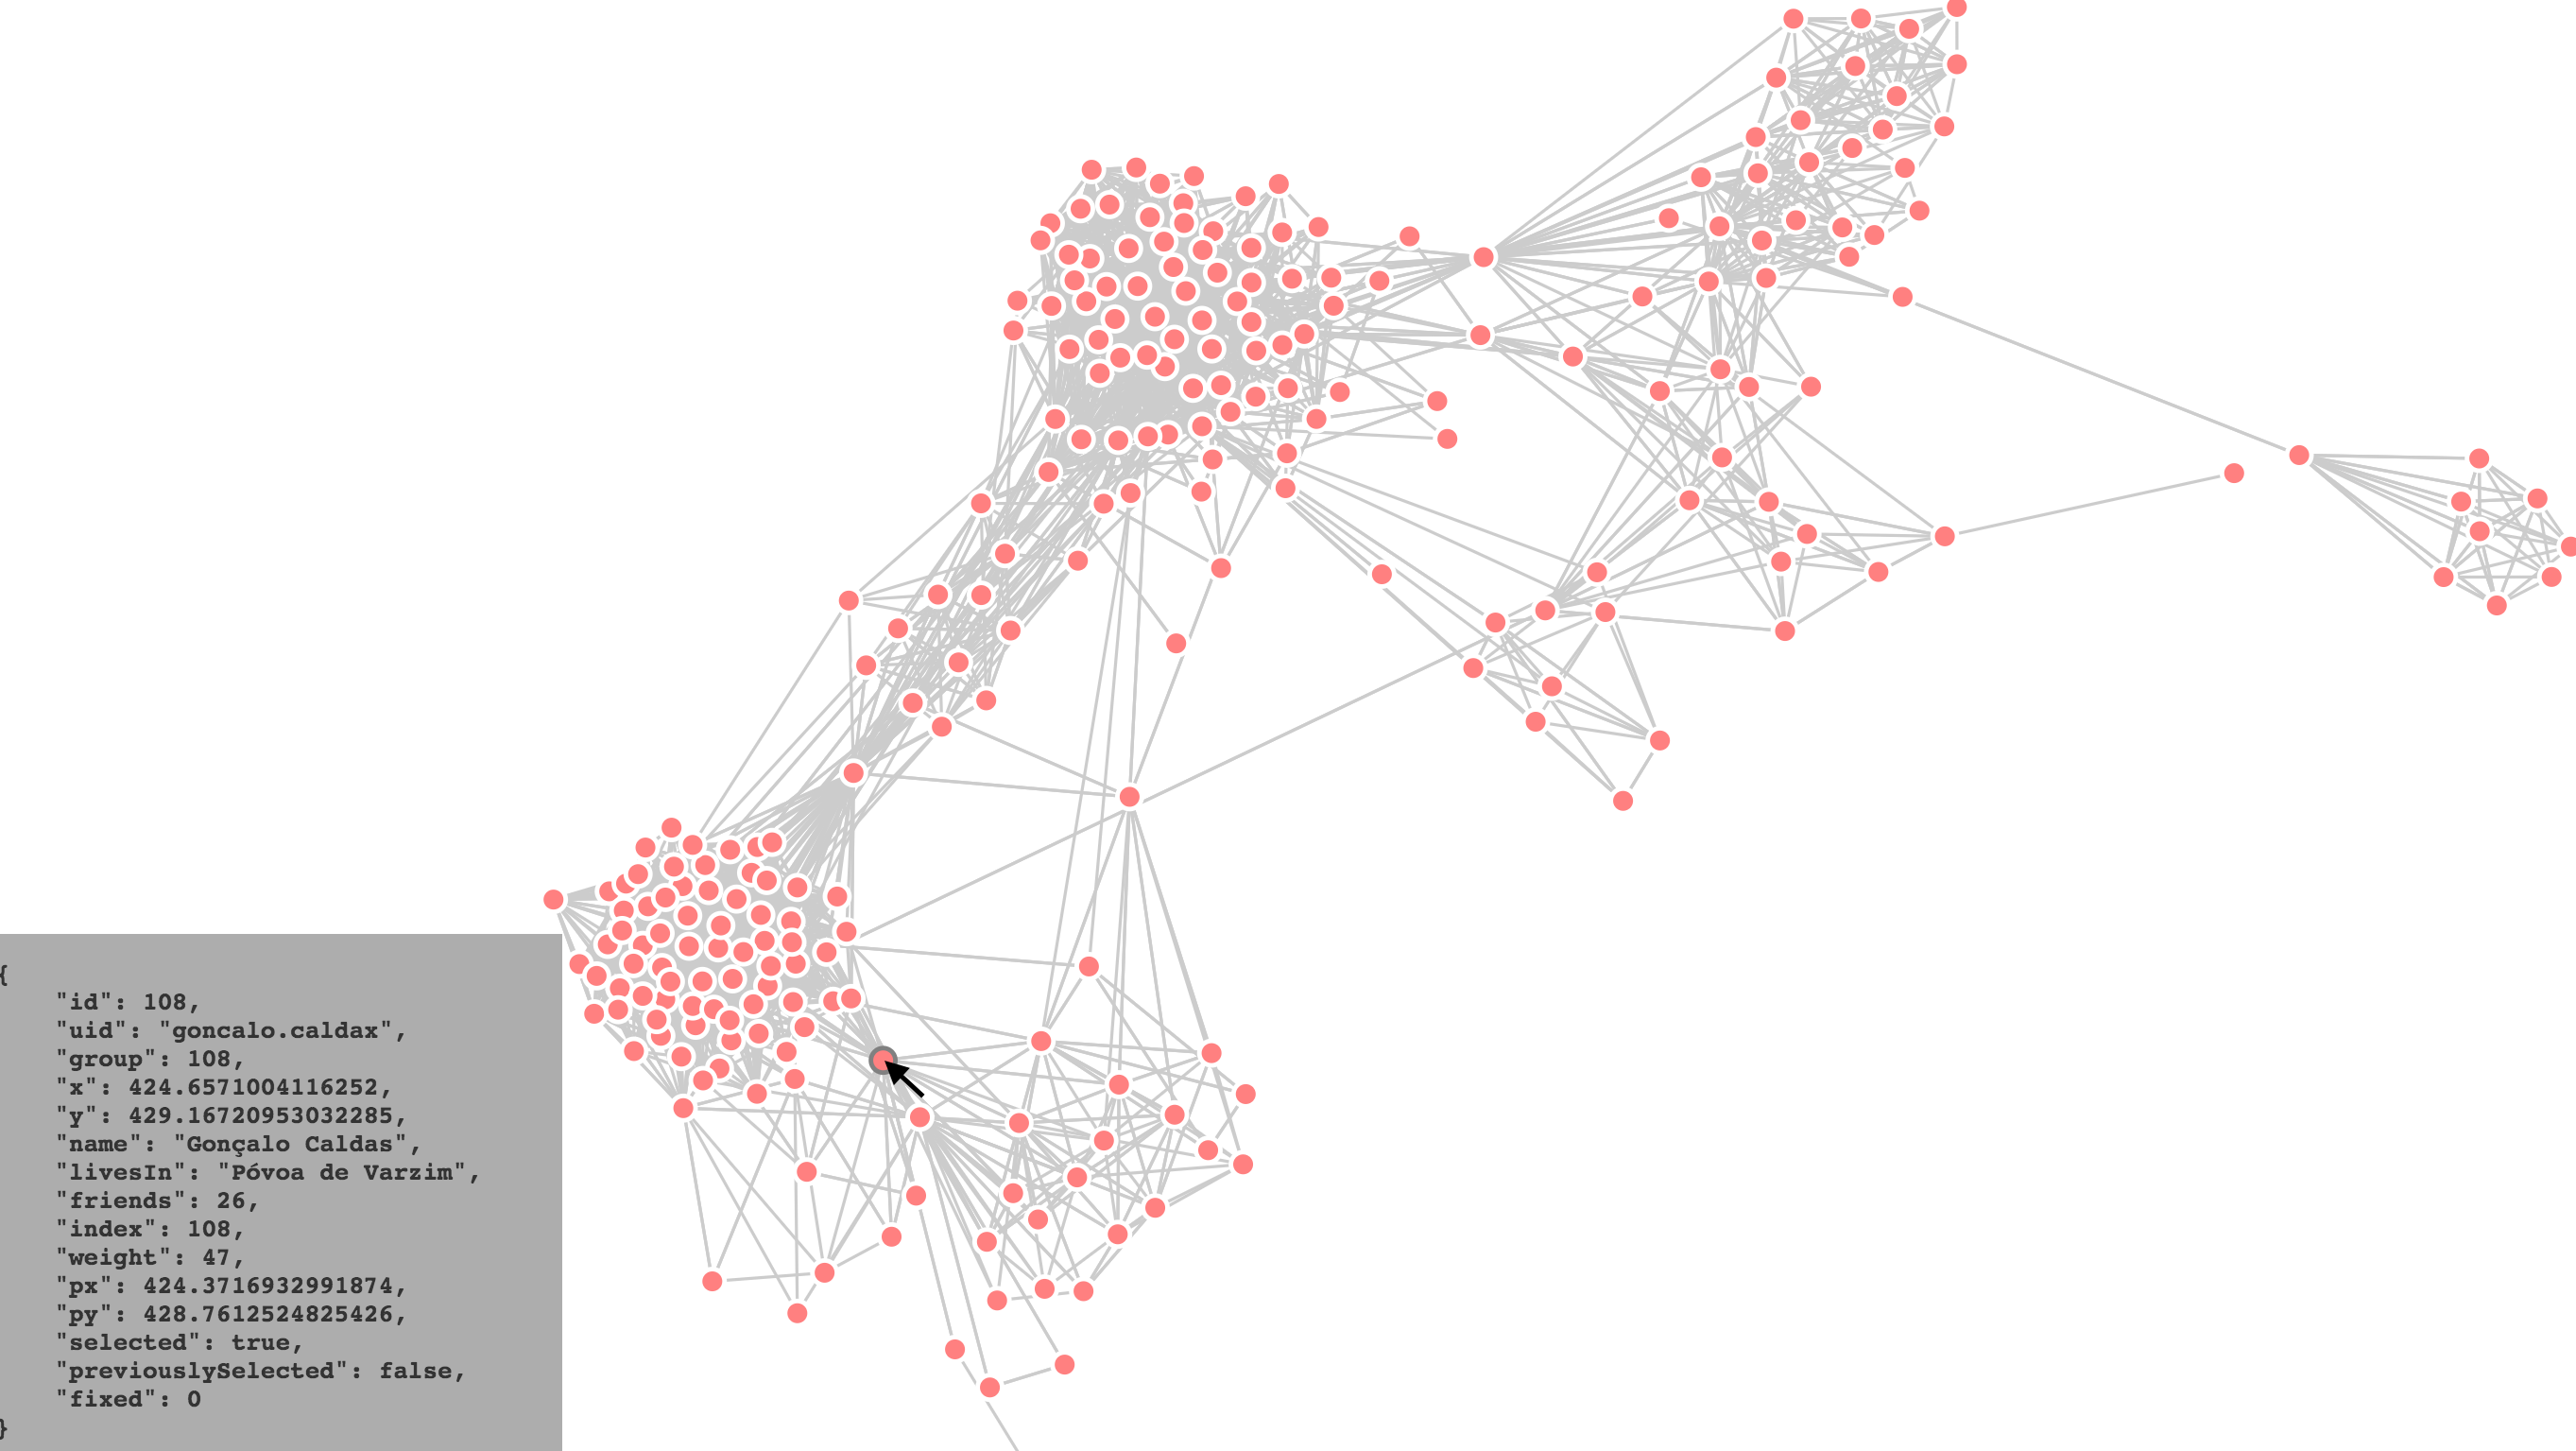
\includegraphics[width=1.2\textwidth]{img/proof-of-concept.png}
\end{center}
\caption{\label{img:poc} A \textit{screenshoot} of our first proof of concept.}
\end{figure}

\indent In in the Figure \ref{img:poc}, we can observe a network being rendered, this represents the friendship network of a given user. Since there is an entry point user, if we let him in this network we would obtain a egocentric network that could not depict all the surrounding relations in these small society. What we did was remove this node order to obtain more clarity to observe the network. At the Figure \ref{img:poc} we also can see the interaction of clicking on a certain node and displaying the node information.

\section{Choose of Technologies}
Having the requirements been defined and a small proof of concept being developed as we seen in the previous section, we are now able to present our technological choices and provide some context on how we came to these conclusions.

\subsection{Database technologies}
(\textbf{MongoDB}, \textbf{Neo4j})\\
Relational databases are one of the complex and advance technologies that we have today. We have been building our applications on top of this technologies with very strict rules that allow our data to remain coherent trough applications lifetimes. Databases engines such as MySQL, PostgresSQL and SQL Server are good live examples of the relevance of this technologies. Meanwhile, applications have grown not just in size but also in complexity, the \textit{web era} came, and with it the need for tools that allow us to manage unstructured data. Other alternatives to relational databases have emerged, this are today known as \textbf{non relational databases} (also known as NoSQL databases). These are database engines that better allow us to store unstructured data or store data in a non relational way. The most suitable NoSQL database in the context of this project are graph databases such as \textbf{Neo4j} (\cite{developers2012neo4j}) that allows to think on data structures as graphs in the the more purest form. Also engines such as \textbf{MongoDB} (a document oriented database, \cite{mongodb}) will give us more flexibility allowing us to have replicated data documents stored in a primary database and then migrate them into a graph database.

\subsection{Back-end technologies}
(\textbf{Python}, \textbf{Flask}, \textbf{Selenium WebDriver}, \textbf{PhantomJS}, \textbf{XPath})\\
The main language that will supports our back-end is Python, this conclusion came very naturally since Python is one of the most used programming languages in the data
science field along with others such as R or Java. We choose Python for two main reasons:
Data extraction and XPath and PhantomJs selenium driver (SEE THIS BETTER)
Network Analysis with Networkx Library

Flask as a simplist framework for building our web \glspl{api} such as extraction and

\subsection{Middleware technologies}
(\textbf{NetworkX}, \textbf{Python}, \textbf{NodeJS})\\
Python should do as well, but since we may want to agelize... We may use modern platforms such as NodeJS that are very well known for
building scalable network applications.

\subsection{Front-end technologies}
(\textbf{HTML}, \textbf{Javascript}, \textbf{CSS}, \textbf{ReactJS}, \textbf{D3.js})\\
\\
Additionally we may add an MVC modern web library such as ReactJS if needed.

In terms of visualization the main Front-end library is D3.js that brings many visualization features out of the box that will help us on
network representation and graph interaction (in the proof of concept we used D3 for rendering the network).

...
\section{Implementation architecture}
...
\section{Implementation details}
...
\subsection{Extraction and data mining}
...
\subsection{Network metrics}
...
\subsection{Front-end and service aggregator}
...
